\documentclass{article}

\usepackage{graphicx}
\usepackage[margin=0.5in]{geometry}

\title{6.111 Final Project Preliminary Report: Real-Time RF Fingerprinting for Amateur Radio Repeaters}
\author{Oliver Trevor}
\date{October 18, 2022}

\begin{document}

\maketitle

\section{Introduction}

The real-time RF fingerprinting system will be called the Radio Society Defense Network externally or the Deparnafier internally (based on a reference to some recent history with repeater trolls). Its purpose is to provide a real-time lockout of unwanted repeater users and realtime identification/logging of legitimate ones' identities. Goals initially include being able to fingerprint (within the time available at the start of a transmission) the number of regular users that the repeater has. Later on, the goal will be to maximize the number of individually-identifiable fingerprints that the system can handle, hoping to reach into the small hundreds.

\section{Feasibility}

\includegraphics[width=5cm]{Yaesu_FT3D_Fingerprint.jpg}

\includegraphics[width=5cm]{Yaesu_FT70D_Fingerprint.jpg}

\includegraphics[width=5cm]{First_Yaesu_FT50_Fingerprint.jpg}

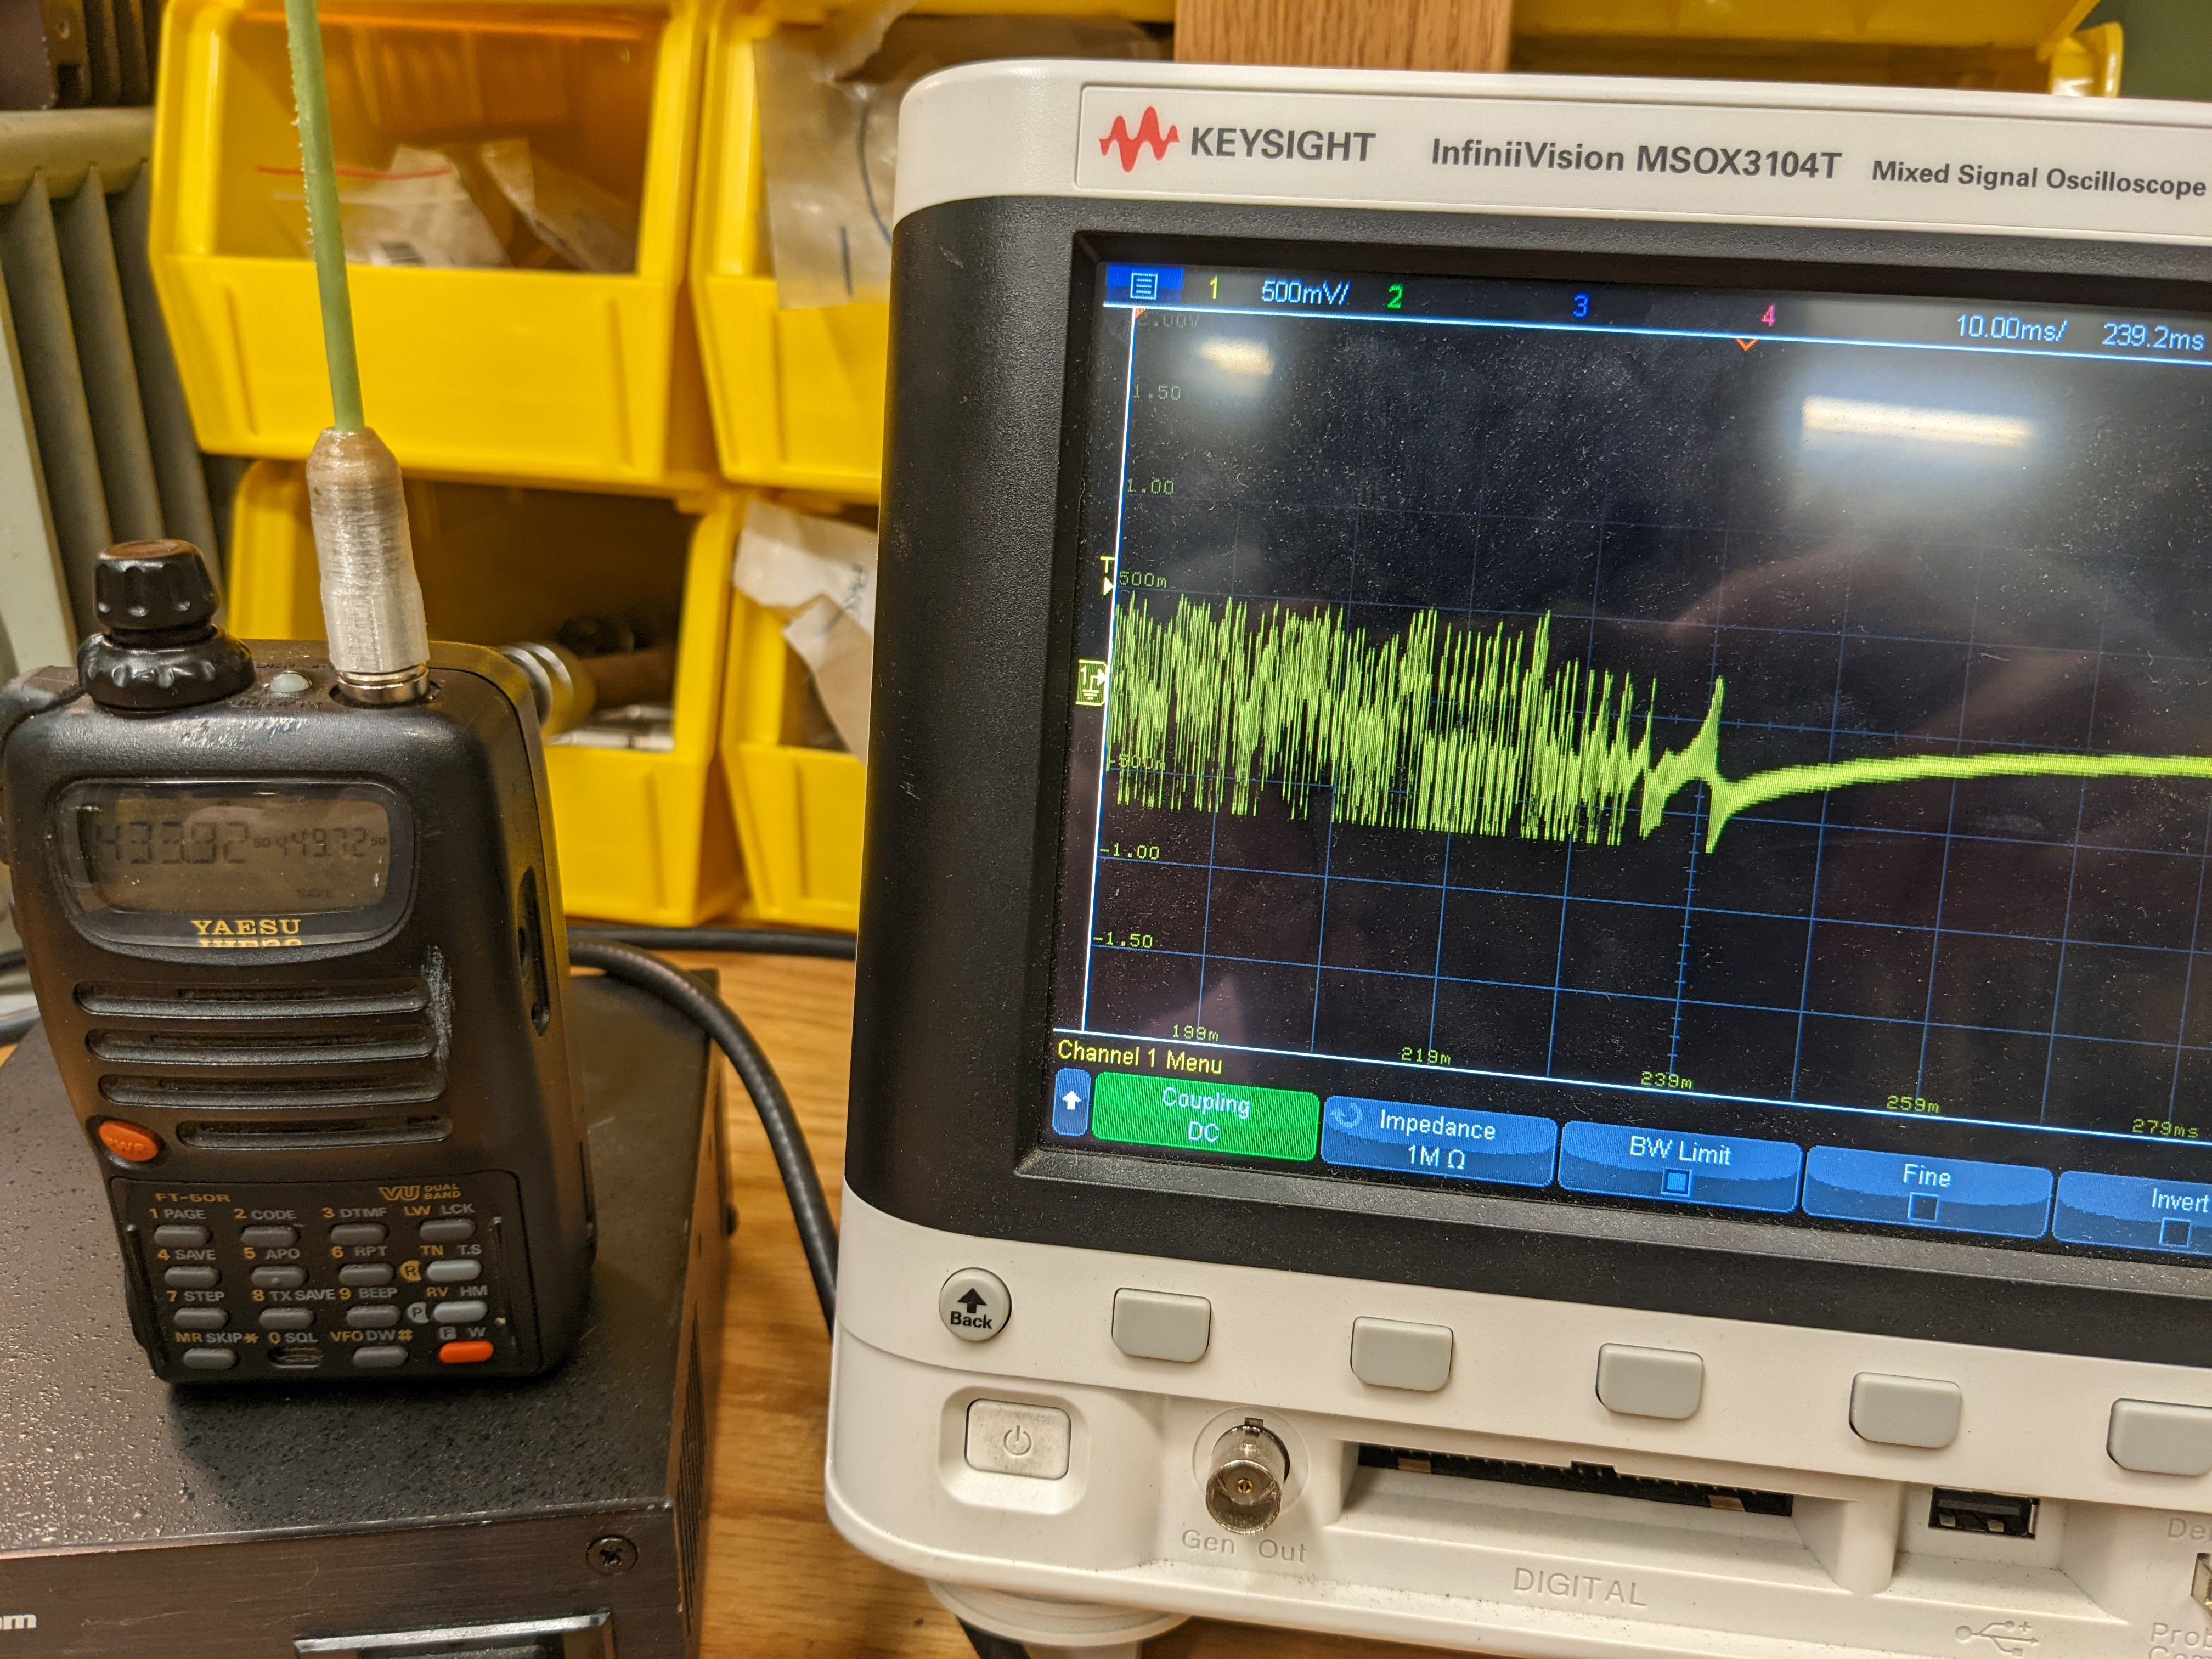
\includegraphics[width=5cm]{Second_Yaesu_FT50_Fingerprint.jpg}

The above photographs show FM discriminator tap recordings taken on a 1 GHz Keysight oscilloscope from the Yaesu FTM-400XDR's DATA jack. Note that all the keyup fingerprint characteristics look significantly different, even for the two Yaesu FT-50's of the same model and age. This suggests that using matched filters to get a strong positive match for identification will be robust.

\section{Design Overview}

\includegraphics[width=8in]{Block_Diagram_Drawing.png}

Data will flow into the system from an external I2S ADC sampling at 10 kSps or higher at 8-bit bit depth (or higher if 8-bit resolution is not available). The data will go into an I2S controller module, which will also handle configuring and bringing up the ADC board. The I2S controller will continuously feed a stream of sample data to the ``start of transmission detector," which lets the system differentiate between random white noise and the start of a transmission.

Note in the earlier FM discriminator recordings that the ``audio" amplitude actually goes \emph{down} upon the start of the transmission due to an effect called \emph{FM quieting} when the incoming signal captures the receiver. Accordingly, to detect an incoming transmission, the detector will use a digital low-pass filter on the incoming signal and detect when the approximate envelope of the signal dips significantly. Depending on how reliably the LPF method is able to trigger on a transmission before the unique portion of the keyup pattern comes in, the system may require a ring buffer so that it can ``go back" a tenth of a second before the actual trigger to avoid the matched filters entirely missing the useful portion of the signal.

Data will then flow into a downsampler to reduce the size of the matched filters and BRAMS necessary to fingerprint the signal. This downsampler is placed after the start-of-TX-detector so that the bandwidth reduction of the downsampler does not drop out some of the white noise that the start-of-TX-detector is triggering on the absence of. Data coming out of the downsampler will be 8-bit signed samples at 10 kSps (or lower if it becomes apparent that high-frequency components do not matter). The downsampler will almost certainly need some internal averaging to act as a rough LPF to prevent aliasing. It may also be possible to entirely remove the downsampler, depending on what datarates the ADC supports and whether the FM quieting can be detected quickly from a slower signal.

The downsampler will feed into the received signal buffer, a 16 kBit BRAM with the ability to be read repeatedly via read lines that come from the filter manager FSM. The job of the received signal buffer is to hold the received signal and feed it into the matched filters repeatedly until there is no processing time left. All matched filters will be fed the same sample at the same time from the received signal buffer, since every matched filter must be tried against the incoming data to find a match.

Depending on how long the convolutions take, each matched filter may actually hold multiple BRAMs of fingerprints internally and compare against more than 1. This is why the received signal buffer needs to exist and be capable of ``resetting" and feeding the same recording more than once. Alternatively, we may choose to trade space for speed and have separate matched filters instantiated for every pattern in memory (depending on how heavy the matched filter logic is, this might be better, since the main resource footprint is BRAM that will have to be consumed by any fingerprint in use no matter how the filters are architectured).

Matched filter modules will perform a convolution of the incoming signal against their stored fingerprint. Parallelizing this effectively and designing it will be most of the complexity of the project. If we choose to use a time-domain convolution, the matched filters will need the received signal buffer to send them the same signal multiple times in order to dot-product the signals at every possible shift between them. If we choose to use a frequency-domain convolution, we may insert a Vivado IP FFT block between the received signal buffer and the matched filter bank, then have the matched filters just perform the convolution by multiplying in the frequency domain. This would, however, require each matched filter to have a separate \emph{inverse} FFT block, so area usage optimization will dictate which of these routes we take.

When a matched filter module finds a match, it will signal the filter manager FSM module with the match (and possibly the match quality, depending on whether we find that signals can have relatively close matches to multiple fingerprints). The filter manager FSM module is in charge of orchestrating the filtering steps, so it controls the read signals to the received signal buffer--and arbitrates which filter's positive match ends up being sent to the output module.

The output module will generate a binary ``transmit enable" signal to the repeater controller as well as sending matches to a computer.

The microSD module will communicate with a microSD card over SPI and load the stored fingerprints into the matched filters' BRAMs at bootup. The data on the microSD card will be raw 8-bit recordings of a fixed length with no filesystem (just written directly to the card starting at address zero and going to address $ N * 16000 $ where $ N $ is the number of stored fingerprints. Since the FPGA can't really ``delete" or ``create" matched filter modules at runtime, $ N $ will be parameterized but fixed at synthesis time. If there are fewer fingerprints than $ N $ stored on the card, the Python script for writing the card will fill that space with 0xFF's so that the matched filters for those empty slots don't match.

\section{Filter Manager FSM}

The filter manager FSM coordinates the high-level operation of the entire process, and it is the only module with a mostly FSM architecture instead of a fully-pipelined one (the uSD controller will probably also contain a large FSM, but this will likely come from a Vivado IP).

\includegraphics[width=6.5in]{FSMs.png}

\section{Other Module Internals}

\includegraphics[width=6.5in]{Modules_1.png}
\newpage
\includegraphics[width=6.5in]{Modules_2.png}
\newpage
\includegraphics[width=6.5in]{Modules_3.png}

\section{Resources}

Each matched filter using design option 1 will require 1 8x8 hardware multiplier. I believe that Vivado is capable of splitting the larger multipliers in the DSP slices into multiple smaller multipliers, so this should be able to efficiently use the DSP slices.

The total number of multipliers used will then be decided by the number of instantiated matched filters, which will be determined by BRAM usage.

Each matched filter needs a 16 kBit BRAM for its own fingerprint. All matched filters share a single receive buffer with a 16 kBit BRAM. So, memory will be internal. I expect BRAM to be the fundamental limiting factor for how many fingerprints we can handle, so BRAM usage will be at or near 100\%.

IPs may be used to perform FFTs and iFFTs if going with option 2 for the matched filters. IPs also may be used to instantiate DSP slice multiply-accumulators explicitly. IPs could also be used to talk to the ADC and uSD card (although these are more likely to be custom).

\section{Conclusion}

This design meets the initial plan in the Abstract to make a system that fingerprints RF keyups in a massively parallel way. This is a uniquely suited problem for an FPGA because matched filtering is very computationally expensive, so the only way to execute many of them in real time is with an FPGA.

Although RF fingerprinting is not new, this is novel because nobody so far has created a real-time system for performing it so quickly as to eliminate interference instead of just policing it retroactively.

The main problem to be resolved is whether to use time-domain or frequency-domain convolution. This will likely be resolved by trying both and seeing how it affects resource usage.

\end{document}
